\subsection{Results and Discussion}
%RHESSI
For a sunquake to be generated by accelerated paticle collision then the incident beam must be aligned over the acoustic impact location \citep{}. To highlight this spatial alignment, RHESSI 50 to 100 keV HXR and sunquake egression power contours are plotted on an IRIS SJI shown in figure \ref{}. %explain alignment of different faetures and the significance      

At the peak of the impulsive phase between 17:46 and 17:47 the RHESSI fit shows an energy ranging from $1.0{\times}10^{28}$ to $2.5{\times}10^{29}$ erg. Assuming the fitting model is correct then the release of this energy is due to non-thermal electrons being accelerated and depositing energy via bremstrahlung collisions in the chromosphere. The nonthermal HXR power signature, $P_e$, can be used to determine the momentum carried by the particle beam producing it by,

\begin{equation}\label{electron-momentum}
p_e=\tau \sqrt{2m_e} P_{e}
\end{equation}

where $m_e$ is electron mass, $\tau$ is the time duration of flare impulsive phase and $P_{e}$ is described by equation \ref{pnth1}. Substituting values in to equation \ref{electron-momentum} yields an electron momentum of $p_e \sim 1.35{\times}10^{17}$ g cm s$^{-1}$. Assuming the energy in the electron beam is equal to that in a population of accelrated protons, then calculation of a theoretical proton beam momentum, where $m_p$ is the proton mass, is by the relation,

\begin{equation}\label{proton-momentum}
p_p \sim p_e \sqrt{frac{m_p}{m_e}}
\end{equation}

Which yields a proton momentum of $p_p \sim 5.79{\times}10^18$ g cm s$^{-1}$, an order of magnitude greater than $p_e$. This is because $m_p ~ 2000m_e$ meaning the square root in equation \ref{proton-momentum} renders the result $p_p \sim 44.7p_e$. So in order to determine whether a particle beam carries enough momentum to stimulate a sunquake, a calculation of the momentum needed to initiated the acoustic response is required. The momentum needed to produce the sunquake is

\begin{equation}\label{sqk-momentum}
p_{sqk}\sim \rho l^{3} v
\end{equation} 

where all terms are tailored for photospheric values, hence density $\rho \sim 10{-8}$g cm$^{-3}$; sound speed $v \sim 10^{6}$ cm.s$^{-1}$. The length-scale, $l \sim  1.82{\times}10_{8}$, corresponds to the sunquake impact diameter, 

\begin{equation}
l = 2\sqrt{\frac{A_{sqk}}{\pi}}
\end{equation}

Equation \ref{sqk-momentum} gives the momentum of the acoustic reponse as $p_{sqk} = 6.03{\times}10^{22}$ g cm s$_{-1}$, which when compared to particle beam momenta, $p_e$ and $p_p, is $10{5}$ and $10^{4}$ times larger respectively. 
This means that even if an electron or proton beam can make it down to the photosphere, it wouldn't have the necessary momentum to cause the sunquake.

%LADDER PLOTS
\begin{figure}[H]
  \begin{center}
  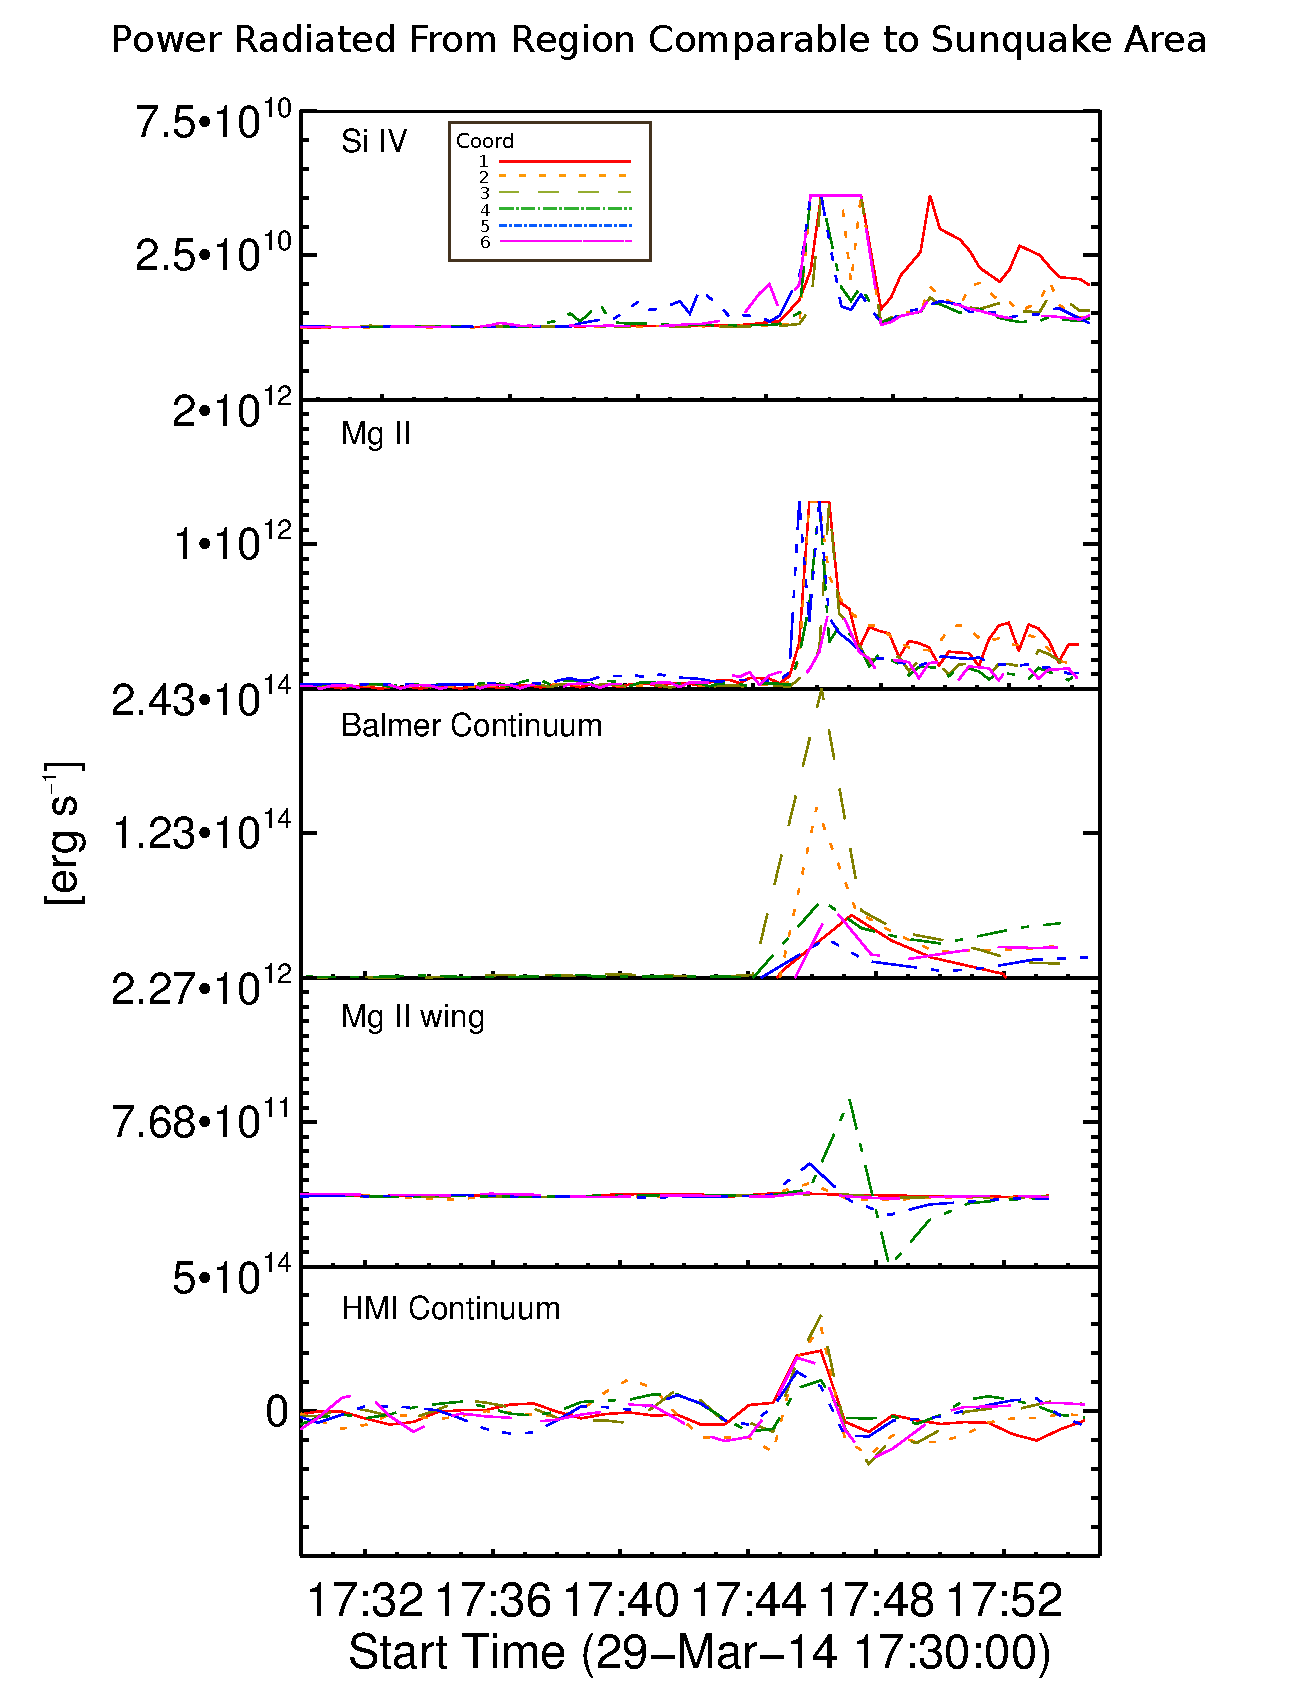
\includegraphics[width=0.6\textwidth]{29-Mar-14-A_sqk-Power-Ladder}
  \end{center}
  \caption{Shows radiative power [erg.s$_{-1}$] from an area comparable to the sunquake impact. The six lines (see legend) represent areas centered on regions 1 to 6, relating to heliocentric coordinates shown in table \ref{}. The solid red line is directly over the sunquake location. Each plot represents an independant data set, in order from top to bottom the sets are; IRIS SJ 1400 \AA\ (Si IV); IRIS SJ 2796 \AA\ (Mg II); IRIS SG  2825.7 to 2825.8 \AA\ (Balmer Continuum); IRIS SJ 2832 \AA\ (Mg II wing); SDO HMI continuum (HMI).}\label{plot1}
\end{figure}



Integrating radiative flux over the impulsive phase of the flare provides an upper limit for energy deposited in the lower atmosphere. The integrated flux is calculated,

\begin{equation}
F_{imp} = \int_{0}^{\tau} F(t) dt = E(t) \tau
\end{equation}
 
where the duration of the impulsive phase $\tau = $ and $F(t)$ is the emitted flux at time $t$. 

$F_{imp}$ can be used to estimate the radiative energy emitted from an area conmparable to $A_{sqk}$ as,

\begin{equation}
E_{imp}=F_{imp}{\times}A_{sqk}
\end{equation}

where it is assumed that a homogenous energy distribution exists throughout the sunquake impact area. This produces values for each data set tabulated in table \ref{eimp}. 

Si IV

Mg II

Balmer continuum

Mg II wing

HMI continuum    


\begin{sidewaystable}[h]\label{eimp}
\tiny
\centering
\begin{tabular}{|c|c|c|c|c|c|c|c|c|c|c|}
Coorinates (x,y) [arcsecs] & $E_{Si IV}$ [erg] & $E_{Mg II}$ [erg] & $E_{Balm}$ [erg] & $E_{Mg II w}$ [erg] & $E_{HMI}$ [erg]\\
\hline
518.22, 262.00 & 6.74E+12 & 1.41E+14 & 5.98E+15 & 4.27E+12 & 1.42E+16\\
520.22, 263.00 & 5.65E+12 & 1.35E+14 & 1.71E+16 & 7.14E+12 & 1.10E+15\\
522.21, 262.00 & 5.18E+12 & 7.83E+13 & 2.52E+16 & 2.91E+12 & 4.82E+15\\
522.21, 265.00 & 3.93E+12 & 8.35E+13 & 9.89E+15 & 6.70E+13 & 1.28E+15\\
524.26, 265.00 & 3.98E+12 & 1.03E+14 & 4.37E+15 & 1.86E+13 & 8.99E+14\\
526.25, 263.82 & 6.91E+12 & 6.34E+13 & 5.24E+15 & 1.74E+12 & 9.88E+14\\
\end{tabular}
\caption{Energies integrated over the flare impulsive phase, 17:44 to 17:48 for ribbon sample locations 1 to 6 (see table \ref{}). E$
\end{sidewaystable}



